\chapter{Computing Background}
\label{TechnologicalBackground}

\begin{quote}
\textit{This chapter presents the current technological state of the art in terms of hardware and software. Hardware-wise, both homogeneous and heterogeneous system architectures and details are presented in sections \ref{HomogeneousSystems} and \ref{HeterogeneousSystems}, respectively. The context of current hardware accelerators is also included in the latter. Software-wise background is presented in section \ref{Software}. Various frameworks and libraries are presented for homogeneous systems and accelerators in early subsections. Section \ref{HeterogeneousFrameworks} presents the available frameworks for parallelization in heterogeneous systems, while current solutions for profiling and debugging parallel applications are presented in section \ref{ProfilingDebugging}.}
\end{quote}

\section{Hardware}
\label{Hardware}

Computer systems originally had a very simple design, where a processing element (in a CPU chip) is connected to a data storage unit (memory). The complexity of the processing chips increased, as well as the memory with the introduction of a cache hierarchy model. Current computing systems are usually made from multicore CPUs, various types of volatile and non-volatile memory and, in some cases, coupled with hardware accelerators.

\subsection{Homogeneous systems}
\label{HomogeneousSystems}

The most common systems are homogeneous, constituted from one or more CPU chips with their own memory bank (RAM memory) and interconnected by a specific interface. Although these systems use a shared memory model, where all the data is shared among CPUs, when considering a multiple CPU system, each has its own memory bank, causing the system to have a Non Unified Memory Access (NUMA) pattern. This means that the access time of a CPU to a piece of memory in its memory bank will be faster than accesses to the other CPU bank. It is important to have the data stored on the CPU memory bank that the application will run to avoid the increased costs of NUMA.

\begin{figure}[!htp]
	\begin{center}
		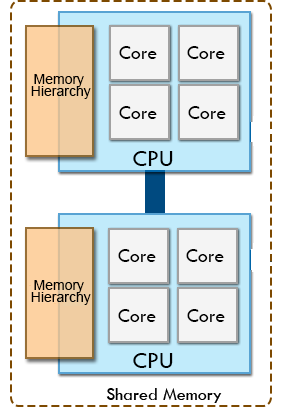
\includegraphics[scale=0.4]{../../common/img/homoplats.png}
		\caption{Schematic representation of a homogeneous system.}
		\label{fig:HomogeneousSystem}
	\end{center}
\end{figure}

Figure \ref{fig:HomogeneousSystem} shematizes the structure of a homogeneous system, in a shared memory environment with the interconnection between CPUs responsible for the NUMA pattern.

\subsubsection*{CPU chips}
\label{CPUChips}

Gordon Moore predicted, in 1965, that for the following ten years the number of transistors on CPU chips would double every 1.5 years \cite{MooreLaw}. This was later known as the Moore's Law and it is expected to remain valid at least up to 2015. Initially, this allowed the increase in CPU chips clock frequency by the same factor as the transistors. Software developers did not spend much effort optimizing their applications and only relied on the hardware improvements to make them faster.

Due to thermal dissipation issues, the clock frequencies of CPU chips started to stall in 2005. Manufacturers shifted from making CPUs faster to increasing their throughput by adding more cores to a single chip, reducing their energy consumption and operating temperature. This marked the beggining of the multicore and parallel computing era, where every new generation of CPUs get wider, while their clock frequencies remain steady.

The CPU chips are designed as general purpose computing devices, based on a simple design consisting of small processing units with a very fast hierarchized memory attached (cache, whose purpose is to hide the high latency access to global memory), and all the necessary data load/store and control units. They are capable of delivering a good performance in a wide range of operations, from executing simple integer arithmetic to complex branching and SIMD (single instruction multiple data, later explained) instructions. A single CPU core implements various mechanisms for improving the performance of applications, at the hardware level, with the most important explained next:

\begin{description}
	\item[\textit{ILP}] instruction level parallelism (ILP) is the overlapping of instructions, performed at the hardware or software level, which otherwise would run sequentially. At the software level it is denominated as static parallelism, where compilers try to identify which instructions are independent, i.e., the result of one does not affect the outcome of the other, and can be executed at the same time, if the hardware has resources to do so. At the hardware level, ILP can be referred as dynamic parallelism as the hardware dynamically identifies which instructions execution can be overlapped while the application is running. Three mechanisms allow for ILP:
	\begin{description}
		\item[\textit{Out of order execution}] is the execution of instructions in different order as they are organized in the application binary, without violating any data dependencies. This technic exposes ILP, which otherwise would not be possible.
		\item[\textit{Super Scalarity}] is a mechanism that allows dispatching a certain amount of instructions to the respective arithmetic units in each clock cycle, increasing the throughput of the CPU. Instructions that are not data dependent can run simultaneously, as long as they use different functional units.
		\item[\textit{Pipelining}] is the division of an instruction execution in stages. The stages range from loading the data, instruction execution in, also pipelined, arithmetic units and writing the results back to memory. For example, this allows for an instruction to be loaded while other is being executed. Moreover, inside an arithmetic unit, multiple instructions can be pipelined, as long as they are in different stages.
	\end{description}
	\item[\textit{Speculative execution}] is the usage of branch prediction, which can use complex algorithms for predicting the conditions, and execute instructions in the predicted branch before knowing the true condition outcome. If the prediction fails, the results are trashed and the other branch is executed. Current hardware is capable of executing both branches of a conditional jump and accept the one correct one once the condition is resolved.
	\item[\textit{Vector instructions}] are a special set of intructions based on the SIMD model, where a single instruction is simultaneously applied to data set. CPU instruction sets offer special registers and instructions that allow to take a chunk of data and execute an instruction to modify it in a special arithmetic unit. One of the most common examples is addition of two vectors. The hardware is capable of adding a given number of elements of the vectors . This optimization is often done at compile time.
	\item[\textit{Multithreading}] is the hardware support for the execution of multiple threads in a core. This is possible by replicating part of the CPU resources, such as registers, and can lead to a more efficient utilization of the CPU core hardware. If one thread is waiting for data to execute the next instruction, other thread can resume execution while the former is stalled. It also allows a better usage of resources that would otherwise be idle during the execution of a single thread. If multiple threads are working on the same data, multithreading can reduce the synchronization between them and lead to a better cache usage.
\end{description}

A schematic representation of a modern CPU chip on its die is presented in figure \ref{fig:CPUChip}. It is constituted of several, possibly multithreaded, cores, each with their own private level 1 and 2 caches and a level 3 cache shared among all cores. This level 3 cache allows fast comunication and synchronization of data between cores of the same CPU.

\begin{figure}[!htp]
	\begin{center}
		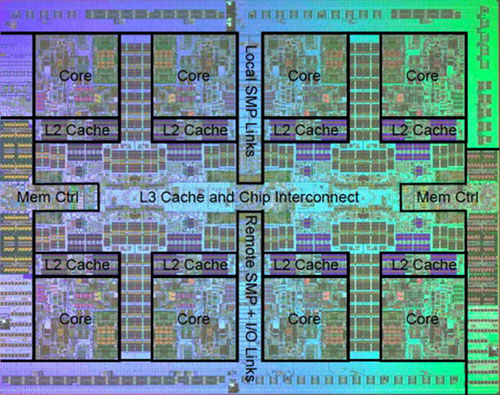
\includegraphics[scale=4]{../../common/img/cpu_scheme.jpg}
		\caption{Schematic representation on a die of a CPU chip.}
		\label{fig:CPUChip}
	\end{center}
\end{figure}

\subsection{Heterogeneous systems}
\label{HeterogeneousSystems}

With the emerging use of hardware specifically designed for some computing domains, denominated hardware accelerators, whose purpose is to efficiently solve a given problem, a new type of computing platform is becoming increasingly popular. This marked the beginning of heterogeneous systems, where one or more CPU chips, operating in a shared memory environment similar to homogeneous systems, are accompanied by one or more hardware accelerators. In current heterogeneous systems, CPUs and accelerators operate in a distributed memory model, meaning that data must be explicitly passed from the CPU to the accelerator, and vice-versa.

\begin{figure}[!htp]
	\begin{center}
		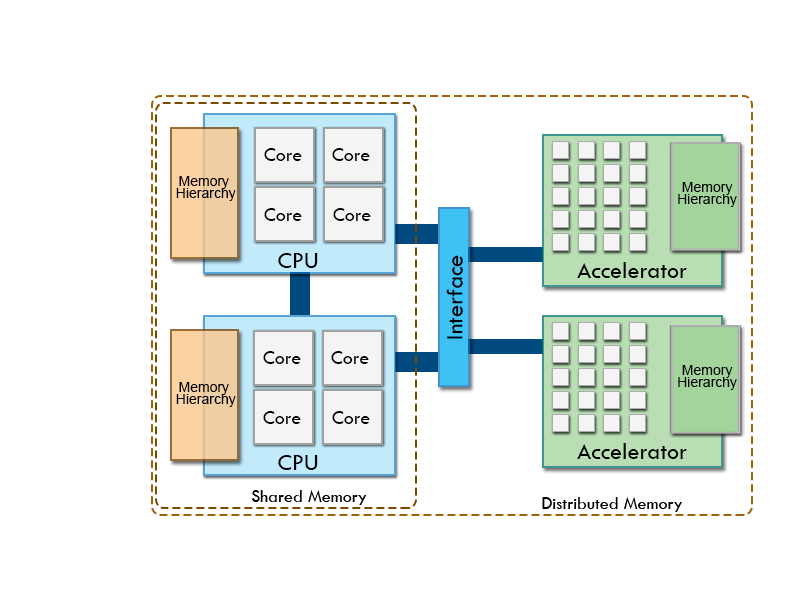
\includegraphics[scale=0.4]{../../common/img/hetplats2.png}
		\caption{Schematic representation of a current heterogeneous system.}
		\label{fig:HeterogeneousSystem}
	\end{center}
\end{figure}

Figure \ref{fig:HeterogeneousSystem} presents a schematic representation of a heterogeneous system. Note that both CPUs must use the same interface to communicate with the hardware accelerators. This interface has a high latency for memory transfers, becoming a potential bottleneck for applications that use accelerators.

Computing accelerators are usually built with a large number of small and simple processing units, aimed to achieve the most performance possible on specific problem domains, as opposed to general purpose CPUs. They are usually oriented for massive data parallelism processing (SIMD architectures), where a single operation is performed on huge quantities of independent data, with the purpose of offloading the CPU from such data intensive operations. Several many-core accelerator devices are available, ranging from the general purpose GPUs to the \intel Many Integrated Core line, currently known as \intel Xeon Phi \cite{Intel:MIC}, and Digital Signal Processors (DSP) \cite{Texas:DSP}. An heterogeneous platform may have one or more accelerator devices of the same or different architectures.

As of June 2013, over 50 of the TOP500’s list \cite{TOP500} are computing systems with hardware accelerators, which indicates an exponential growth in usage compared to previous years. The \intel Xeon Phi is becoming increasingly popular, being the accelerator device of choice in 11 clusters of the TOP500. \nvidia GPUs remain as the most used accelerator.

\subsubsection*{Graphics Processing Unit}
\label{GPU}

The Graphics Processing Units (GPU) were one of the first hardware accelerators on the market. Their purpose is to accelerate computer graphics applications, which started of as simple pixel drawing and evolved to support complex 3D scene rendering, such as transforms, lighting, rasterization, texturing, depth testing, and display. Due to the industry demand for costumizable shaders, this hardware later allowed some flexibility for the programmers to modify the image synthesing process. This also allowed using this GPUs as a hardware accelerator for wider purposes beyond computer graphics, such as scientific computing.

The GPU architecture is based on the SIMD model. Its original purpose is to process and synthethise images, which are, computationally, a large set of pixels. The processing of each pixel usually does not depend on the processing of its neighbours, or any other pixel on the image, making the process data independent. This allows for processing the pixels simultaneously. The massive data parallelism is one of the most important factors that molded the design of the GPU architecture.

As the GPU manufacturers allowed more flexibility to program their devices, the High Performance Computing (HPC) community started to use them to solve specific massively data parallel problems. One of the most known examples is matrix algebra, such as additions and multiplications. However, GPUs had some important features only oriented for computer graphics that affected its use in other situations. One example is that initially the GPU only supported single precision floating point arithmetic. Due to the increase demand for these devices by the HPC community, manufacturers began to generalize more of the GPUs features, such as supporting double precision floating point arithmetic, and later began producing accelerators specificaly oriented for the scientific computing. \nvidia is the number one GPU manufacturer for scientific computing GPUs, with a wide range of available hardware known as the Tesla. These devices have more GDDR RAM, processing units and a slightly different structural design suitable for use in cluster computational nodes, with a different size and cooling mechanisms. The chip architecture suffered some changes too, increasing the cache size and the amount of processing units. The \nvidia Tesla C2070 (based on the Fermi architecture \cite{NVIDIA:Fermi}) was used during this dissertation work.

The \nvidia GPU architecture has two main components: computing units (Streaming Multiprocessors, also known as SM) and the memory module (global external memory, GDDR5 RAM, and a 2-level in-chip cache and shared memory block). Each SM contains a set of CUDA cores, \nvidia designation for their basic processing units that perform both integer and float point arithmetic (additions, multiplications and divisions). These SMs also have some specialized processing units for square root, sins and cosines computation, as well as a warp scheduler (warps are later explained) that matches the CUDA threads to CUDA cores, load and store units, register files and the L1 cache/shared memory. The L2 cache is shared among all SMs in a GPU chip.

A warp is a set of CUDA threads (it has a size of 32 CUDA threads in the Fermi architecture), scheduled by the SM scheduler to run on its SM at any given time, out of a pool with 48 warps ready to rin. A warp can only be constituted by CUDA threads from the same block\footnote{The GPU thread hierarchy and organization is presented in section \ref{CUDA}.}.

Accesses to the GPU global memory have a high latency that can cause the CUDA threads to be stalled waiting for data. The strategy behind the GPU architectures is to provide the device with a huge amount of threads, allowing the schedulers to keep a scoreboard of which warps are ready to execute and which are waiting for data to load. This grants the scheduler with enough threads to always have a warp ready for execution, preventing the starvation of the SMs.

Since the GPU is connected by PCI-Express interface, the bandwidth for communications between CPU and GPU is restricted to only 12 GB/s (6 GB/s in each direction of the channel). Memory transfers between the CPU and GPU must be minimal as it greatly restricts the performance.

\begin{figure}[!htp]
	\begin{center}
		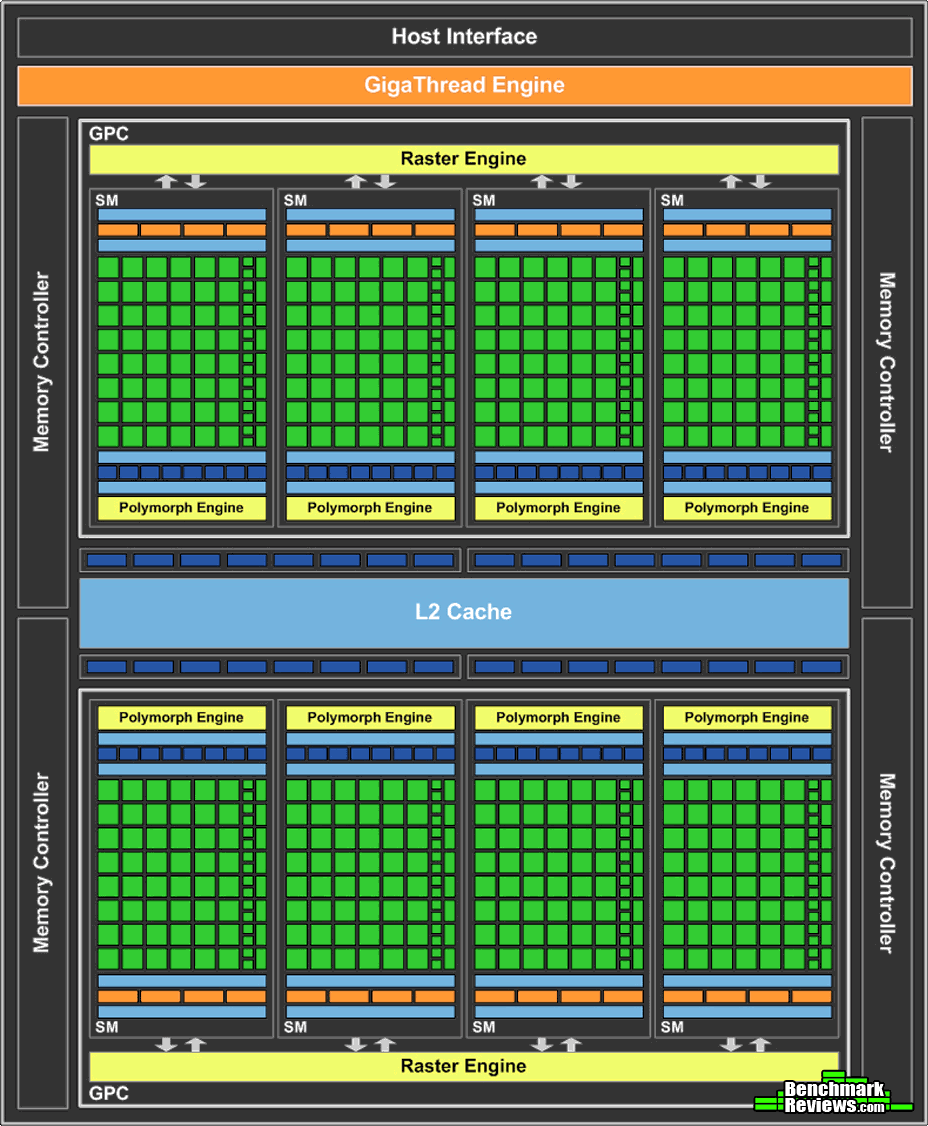
\includegraphics[scale=0.3]{../../common/img/fermi_arch.png}
		\caption{Schematic representation of the \nvidia Fermi architecture.}
		\label{fig:FermiArchitecture}
	\end{center}
\end{figure}

In the Tesla C2070, with its architecture shown in figure \ref{fig:FermiArchitecture}, each one of the 14 SM in the chip have 32 CUDA, making a total of 448 CUDA cores. Each SM has 4 Special Functional Units (SFU) to process special operations such as square roots and trignometric arithmetic.

These devices have a slightly different memory hierarchy than CPUs, but still with the faster and smaller memory closer to each processing unit (SM). Each CUDA thread can use up to 63 registers, but decreasing with the amount of threads used, which can, in some cases, lead to register spilling (when there is not enough registers to hold the variables values and they must be stored in high latency global memoy).

Within each SM there is a block of configurable 64 KB memory. In this architecture it is possible to use it as 16 KB for L1 cache and 48 KB for shared memory (only shared between threads of the same block), or vice-versa. The best configuration is dependent of the specific characteristics of each algorithm, and usually requires some preliminary tests to evaluate which configuration obtains the best performance. Shared memory can also be used to hold common resources to the threads, even if they are read-only, avoiding accesses to the slower global memory. The L2 cache is slower but larger, 768 KB, shared among all SMs. The Tesla C2070 has a total of 6 GB GDDR5 RAM, with a bandwidth of 192.4 GB/s.

One important detail for efficient memory usage is the control of coalesced memory accesses. As the load units fetch memory in blocks of 128 bits, it is possible to reduce the amount of loads by synchronizing and grouping threads that need to load data which is in contiguous positions. This grouping is made by the memory controller, but only if the threads need the contiguous data simultaneously.

\subsubsection*{Intel Many Core architecture}
\label{MIC}

The \intel Many Integrated Core (MIC) architecture, with the current production device known as Intel Xeon Phi, has a different conceptual design than the \nvidia GPUs. A chip can have up to 61 multithreaded cores, with 4 threads per core. Rather than extract performance by resorting to massive parallelism of simple tasks, the design favours vectorization as each core has 32 512 bit wide vector registers \cite{Intel:MIC}.

\begin{figure}[!htp]
	\begin{center}
		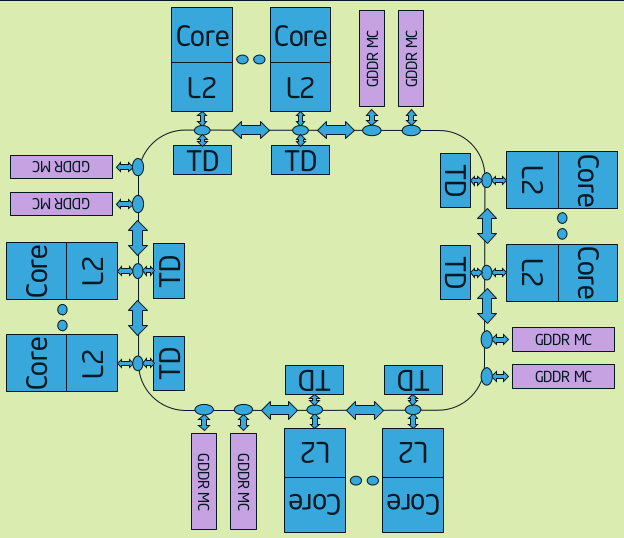
\includegraphics[scale=0.5]{../../common/img/mic_arch.png}
		\caption{Schematic representation of the \intel MIC architecture.}
		\label{fig:MICArchitecture}
	\end{center}
\end{figure}

The vector registers can hold 16 single precision float point values. Each core has L1 cache with a size of 64 KB for data and 64 KB for instructions, and 512 KB L2 cache. There is no shared cache between the cores inside the chip. The device board has 6 or 8 GB GDDR5 RAM, with a maximum bandwidth of 320 GB/s. Its design is more oriented for memory bound algorithms, as opposed to GPUs (Fermi only has a bandwidth of 192.4 GB/s). \intel claims that it will later launch a device tuned for compute bound problems.

Unlike conventional CPUs, the MIC cores do not share any cache, therefore cache consistency and coherence is not ensured by the hardware. It works as a distributed memory system, but consistency can be ensured by software, with a high latency. The cores are connected in a bidireccional ring network, as represented in figure \ref{fig:MICArchitecture}. The MIC uses the same instruction set as conventional x86 CPUs. Intel claims that this allows to easily port current applications and libraries to run on this device.

The MIC architecture has some simplifications compared to the CPU architecture, so that it is possible to fit so many cores inside a single chip. MIC does not support out of order execution, which greatly compromises the use of ILP. Also, the clock frequency is limited to 1 GHz, less than half of the modern CPUs.

The Xeon Phi has two operating modes:

\begin{description}
	\item[Native:] the device acts as system itself, with one core reserved for the operative system. The application and all libraries must be compiled specifically to run on the device, as well as copied to the its memory, along with the necessary input data, prior to execution. No further interaction with the CPU is required.
	\item[Offload] the device acts an accelerator, accessory to the CPU. Only part of the application is set to run on the Xeon Phi, and data must be explicitly passed between CPU and device each time code will execute in it. All library functions called inside the device must be explicitly compiled and it is not possible to have an entire library compiled simultaneously for the Xeon Phi and CPU.
\end{description}

\subsubsection*{Other hardware accelerators}
\label{OtherAccelerators}

More hardware accelerators are coming to the market due to the increasingly popularity of GPUs and \intel MIC among the HPC community. Texas Instruments developed their new line of Digital Signal Processors, best suited for general purpose computing while very power efficient. Their capable of delivering 500 GFlop/s (giga float pointing operations per secong), consuming only 50 Watts \cite{Texas:DSP}.

ARM processors are now leading the mobile industry and, alongside the new \nvidia Tegra processors \cite{NVIDIA:Tegra} that are steadly increasing their market share, are likely to be adopted by the HPC community\footnote{e.g. the ARM based Montblanc project will replace the MareNostrum in the Barcelona Supercomputing Center (BSC)} due to their low power consumption while delivering high performance \cite{ARM}. The shift from 32-bit to 64-bit mobile processors is happening due to the increase in complexity of mobile systems and applications.

\section{Software}
\label{Software}

Most programmers are only used to code and design sequential applications, showing a lack of know-how to develop algorithms for parallel environments. This issue is even greater when considering heterogeneous systems, where programming paradigms shift when considering different hardware accelerators. The mainstream industry is still adopting the use of multicore architectures with the purpose of increasing their processing power, causing a lack in the academic training of programmers in terms of optimization and parallel programming. Self taught programmers have an increased obstacle due to the lack of theoretical basis when using these new parallel programming paradigms.

Programming for multicore environments requires some knowledge of the underlying architectural concepts. Shared memory, cache coherence and consistency and data races are architecture-specific aspects that the programmer does not face in sequential execution environments. However, these concepts are fundamental not only to ensure efficient use of the computational resources, but also the correctness of the application.

Heterogeneous systems combine the flexibility of multicore CPUs with the specific capabilities of many-core accelerator devices, connected by PCI-Express interfaces. However, most computational algorithms and applications are designed with the specific characteristics of CPUs in mind. Even multithreaded applications usually cannot be easily ported to these devices expecting high performance. To optimize the code for these devices it is necessary a deep understanding of the architectural principles behind their design.

The most important aspect to ensure the correcteness of an application on a shared memory environment is to control data races, i.e., concurrent accesses of different threads to shared data. As an example, when modifying shared data, the programmer must ensure that different threads are not simultaneously changing the same piece of memory by serializing the operations. Further control is required if the order of the operations is important. If one thread wants to change a piece of data while other wants to read it, it is necessary to define which of the threads has the priority, as it can affect the outcome of the rest of both threads operations.

The workload balance between the cores of a single CPU chip is an important aspect to extract performance and get the most efficient usage of the available resources. A inadequate workload distribution may cause some cores of the CPU to be used most of the time while others remain idle, making the application to take more time than necessary to execute. A good load balancing strategy ensures that all the cores are used as most as possible. Considering a multi-CPU system, it is important to manage the data in such a way that it is available in the memory bank of the CPU that will need it to avoid the NUMA latency. The same concepts apply when balancing the load between CPU and hardware accelerators, with the increased complexity of the high latency data transfers of the PCI-Express interface.

Some computer science groups developed libraries that attempt to abstract the programmer from specific architectural and implementation details of these systems, providing an easy API as similar as possible to current sequential programming paradigms. Some frameworks that attempt to abstract the inherent complexity of heterogeneous systems are already in the final stages of development.

\subsection{Shared memory environment}

Homogeneous systems often operate in a shared memory environment. Using multiple CPUs may cause the memory banks to be physically divided but hardware mechanisms, such as CPU interconnections, allow for a common addressing space. Libraries and frameworks for parallelizing for this environment are presented next.

\subsubsection*{pThreads}
\label{pThreads}

Threads are the base unit that can be scheduled by the operating system. POSIX Threads (pThreads) are the standard implementation for UNIX based operating systems with POSIX conformity, such as most Linux distributions and Mac OS. The pThreads API provides the user with primitive for thread management and synchronization. Since this API forces the user to deal with several implementation details, such as data races and deadlocks, the industry demanded the development of high level libraries, which are usually based on pThreads.

\subsubsection*{OpenMP, TBB and Cilk}
\label{OpenMP}

OpenMP \cite{OpenMP}, \intel Threading Building Blocks (TBB) \cite{Intel:TBB} and Cilk \cite{Cilk} are the response for the industry demands for a higher abstraction level APIs.

The OpenMP API is designed for multi-platform shared memory parallel programming in C, C++ and Fortran, on all available CPU architectures. It is portable and scalable, aiming to provide a simple and flexible interface for developing parallel applications, even for the most inexperienced programmers. It is based in a work sharing strategy, where a master thread spawns a set of slave threads and compute a task in a shared data structure.

\intel TBB employs a work stealing heuristic, where if the task queue is empty a thread attempts to steal a task from other busy threads. It provides a scalable parallel programming task based library for C++, independent from architectural details, only requiring a C++ compiler. It automatically manages the load balancing and some cache optimizations, while offering parallel contructors and sychronization primitives for the programmer.

Cilk is a runtime system for multithreading programming in C++. It maintains a stack with the remaining work, employing a work stealing heuristic very similar to Intel TBB.

\subsection{Distributed memory environment}
\label{HeterogeneousFrameworks}

Heterogeneous systems use distributed memory address space for handling the data between CPU and accelerator device. Even though the CPUs work on a shared memory space, data must be explicitly passed to the accelerators. Frameworks for parallelizing on the devices and on the heterogeneous platforms as a whole are presented next.

\subsection*{Message passing interface}
\label{MPI}

The Message Passing Interface (MPI) \cite{MPI}, designed by a consorcium of both academic and industry researchers, has the objective of providing a simple API for parallel programming in distributed memory environments. It relies on point-to-point and group messaging communication, and is available in Fortran and C. The data must be explicitly split and passed among the processes by the programmer. It is often used in conjunction with a shared memory parallel programming API, such as OpenMP, for work sharing between computing nodes, with the latter ensuring the parallelization inside each node.

\intel adapted an MPI version to work on both CPUs and Xeon Phi, considering the device as a set of CPUs. Comunications between the CPU and device are explicitly handled by the programmer. The other method for working with this device is to use compiler directives for data communication and code parallelization.

\subsubsection*{CUDA}
\label{CUDA}

The Compute Unified Device Architecture (CUDA) is a computing model for hardware accelerators launched in 2007 by \nvidia. It aims to provide a framework for programming devices similar architecture to the \nvidia GPUs. It has a specific instruction set architecture (ISA) and allows programmers to use GPUs for other purposes than image rendering.

\nvidia considers that a parallel task is constituted by a set of CUDA threads, which execute the same instructions (conditional jumps are a special case that will be later explained) but on different data. This set of instructions is considered a CUDA kernel, in which the programmer defines the behavior of the CUDA threads. A simple way to visualize this concept is to consider the example of multiplying a scalar with a matrix. In this case, a single thread will handle the multiplication of the scalar by an element of the matrix, and it is needed to use as many CUDA threads as matrix elements.

The CUDA thread is the most basic data independent parallel element, which can run simultaneously with other CUDA threads but itself cannot be parallelized, and is organized in a hierarchy presented in figure \ref{fig:CUDAHierarchy}. A block is a set of CUDA threads that is matched by the global scheduler to run on a specific SM. A grid is a set of blocks, representing the whole parallel task. Considering the matrix example, each CUDA thread corresponds to an element of the matrix, computing its value, and is organized in a block of many CUDA threads that can represent all the computations for a single line of the matrix. The grid holds all the blocks responsible for computing all the new values of the matrix. Note that both the blocks and the grid have a limited size.

\begin{figure}[!htp]
	\begin{center}
		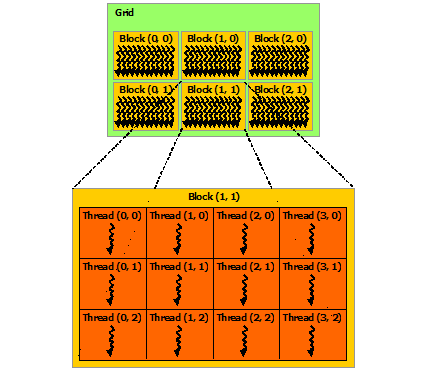
\includegraphics[scale=0.9]{../../common/img/cuda_hierarchy.png}
		\caption{Schematic representation of CUDA thread hierarchy.}
		\label{fig:CUDAHierarchy}
	\end{center}
\end{figure}

When programming these devices, conditional jumps must be avoided if they cause different CUDA threads within the same warp execute different branches. Within an SM it is not possible to have 2 threads executing different instructions at the same time. So, if there is a divergence between the threads within the warp, the divergent branches will be executed sequentially, doubling the warp execution time.

\subsubsection*{OpenACC}
\label{OpenACC}

OpenACC \cite{OpenACC} is a framework for heterogeneous platforms with accelerator devices. It is designed to simplify the programing paradigm for CPU/GPU systems by abstracting the memory management, kernel creation and GPU management. Like OpenMP, it is designed for C, C++ and Fortran, but allowing the parallel task to run on both CPU and GPU at the same time. However, it does not schedule the load between the CPU and GPU.

While it was originally designed only for CPU/GPU systems, they are currently working on the support for the new \intel Xeon Phi \cite{OpenACC:HPCWire}. Also, they are working alongside with the members of OpenMP to create a new specification supporting accelerator devices in future OpenMP releases \cite{OpenACC:OpenMP}.

\subsubsection*{GAMA}
\label{GAMA}

The GAMA framework \cite{GAMA} has a similar goal to OpenACC, to provide the tools to help building efficient and scalable applications for heterogeneous platforms, but follows a different approach. It aims to create an abstraction layer between the architectural details of heterogeneous platforms and the programmer, aiding the development of portable and scalable parallel applications. However, unlike OpenACC, its main focus is on obtaining the best performance possible, rather than abstracting all the architecture details from the programmer. The programmer still needs to have some knowledge of each different architecture, and it is necessary to instruct the framework about how tasks should be divided in order to fit the requirements of the different devices.

The framework frees the programmer from managing the workload distribution (apart from the dataset division), memory usage and data transfers between the available devices. However, it is possible for the programmer to tune these specific details, if he is confortable enough with the framework.

GAMA assumes a hierarchy composed of multiple devices (both CPUs and GPUs, in its terminology), where each device has access to a private address space (shared within that device), and a distributed memory system between devices. To abstract this distributed memory model, the framework offers a global address space. However, since the communication between different devices is expensive, GAMA uses a relaxed memory consistency model, where the programmer can use a synchronization primitve to enforce memory consistency.

\subsection{Profiling and debugging}
\label{ProfilingDebugging}

\subsubsection*{VTune}
\label{VTune}

Intel VTune profiler \cite{Intel:VTune} is a proprietary tool for performance analysis of applications. It provides an easy to use tool which analyzes the applications, identifying its bottlenecks, without any change to the source code. VTune also provides visualization functionalities making profiling of parallel applications a simple task for developers with small experience.

\subsubsection*{Performance API}
\label{PAPI}

The Performance API (PAPI) \cite{PAPI} specifies an API for hardware performance counters in most modern processors. It allows programmers to measure the performance counters for specific regions of an application, evaluating metrics such as cache misses, operational intensity or even power consumption. This analysis helps classifying the algorithms and identify possible bottlenecks at a very low abstraction level.

\subsubsection*{Debugging}
\label{Debugging}

Debugging applications in shared memory systems is a complex task, as the errors are usually harder to replicate than on sequential applications. Bugs can happen due to deadlocks, unexpected changes to the shared memory, data inconsistency and incoherence. While there are some tools to efficiently debug sequential applications, such as the GNU Debugger \cite{GDB}, they lack on the support for multithreaded applications. Unfortunately, there are no debuggers that can efficiently be used to debug a parallel application.

The effort necessary to debug these applications, without the use of any third-party tools, is directly related to the programmers experience and knowledge of working with shared memory systems. However, even the most experienced will face complex obstacles when debugging for more than 4 threads, as the application behavior is much harder to control.

Nvidia offers a tool for debugging CUDA kernels on their GPUs, which is based on the GNU Debugger \cite{NVIDIA:gdb}. It is useful when used to find bugs in the kernels, but only in the same way that a sequential application is debugged. Also, when using more than 2-4 CUDA threads it does not help the programmer at all, considering that CUDA kernels can reach to the thousands of threads.
